% mainfile: ../../main.tex
\chapter{Optical path}\label{ch:setup:optics}
\AutoLettrine{The} confocal microscope integrated into a millikelvin-temperature cryogen-free \gls{dr} accommodating free-space optical measurements together with DC and AC electrical control was designed and set up by \citeauthor{Descamps2024}~\cite{Descamps2021,Descamps2024}.
In this chapter, I lay out improvements to the design to improve the optical efficiency of the microscope.
I review the relevant relationships between optical parameters, estimate the maximum expected efficiency, and compare it to measurements.
Furthermore, I characterize the cross-polarization extinction and outline various schemes I established to automatically control the motorized stages regulating the excitation power and rejection as well as the diffraction grating spectrometer and \gls{ccd}.
Lastly, I demonstrate the setup's efficacy to measure photon anti-bunching in a \g2 measurement on self-assembled quantum dots in \ch{InGaAs}.

\begin{marginfigure}[*-8]
    \begin{tikzpicture}[
    scale=2,%
    font=\footnotesize,%
    thick,%
    symmetryaxis/.style = {RWTHblack50,thin,dash dot},%
    lens/.style = {thick,<->},%
    optics/.style = {thick,black},%
    window/.style = {RWTHblue75,fill=RWTHblue25,text=black,opacity=0.75},%
    cryostat/.style = {RWTHblack75,thin,text=black},%
    midarrow1/.style = {postaction=decorate, decoration={markings,mark=at position 0.15 with \arrow{stealth}}},%
    midarrow2/.style = {postaction=decorate, decoration={markings,mark=at position 0.85 with \arrow{stealth}}},%
    midarrow/.style = {midarrow1, midarrow2},%
]    % requires libraries angle,quotes,calc,decorations.markings

    \ifdefined\CA
    \else
        \newlength\CA
    \fi
    \ifdefined\f
    \else
        \newlength\f
    \fi
    \ifdefined\dx
    \else
        \newlength\dx
    \fi
    \setlength\CA{0.25cm}
    \setlength\f{0.4cm}
    \setlength\dx{0.25cm}

    \coordinate (origin) at (0, 0);
    \coordinate (bs1) at (0, 0);
    \coordinate (bs2) at (0, -1);
    \coordinate (window) at ($(bs2) + (0, -0.8)$);
    \coordinate (objective) at ($(window) + (0, -1.5)$);

    \coordinate (detection-halfwave) at ($(bs1) + (0, 0.6)$);
    \coordinate (analyzer) at ($(detection-halfwave) + (0, 1*\dx)$);
    \coordinate (detection-ocular) at ($(detection-halfwave) + (0, 2*\dx)$);

    \coordinate (quarterwave) at ($(bs1) + (0.6, 0)$);
    \coordinate (excitation-halfwave) at ($(quarterwave) + (1*\dx, 0)$);
    \coordinate (polarizer) at ($(quarterwave) + (2*\dx, 0)$);
    \coordinate (excitation-ocular) at ($(quarterwave) + (3*\dx, 0)$);

    \coordinate (cmos-ocular) at ($(bs2) + (0.6, 0) + (3*\dx, 0)$);

    \coordinate (source) at ($(objective) - (0, \f)$);
    \coordinate (detection-fiber) at ($(detection-ocular) + (0, \f)$);
    \coordinate (excitation-fiber) at ($(excitation-ocular) + (\f, 0)$);
    \coordinate (cmos) at ($(cmos-ocular) + (\f, 0)$);

    % Symmetry axes
    \draw[symmetryaxis]
        ($(bs1) - (\CA*2,0)$)
        -- ($(excitation-fiber) + (\f/4,0)$)
    ;
    \draw[symmetryaxis]
        ($(bs2) - (\CA*2,0)$)
        -- ($(cmos) + (\f/4,0)$)
    ;
    \draw[symmetryaxis]
        ($(source) - (0, \f/4)$)
        -- ($(detection-fiber) + (0, \f/4)$)
    ;

    % Cryostat
    \draw[cryostat]
        ($(window) - (1.5*\CA, -0.025)$)
        -- ++($(-\f/2, 0)$)
        -- ($(source) - (1.5*\CA + \f/2, \f/2)$)
        -- ++($(3*\CA + \f, 0)$)
        -- ($(window) + (1.5*\CA + \f/2, 0.025)$) node[below,midway,rotate=90,xshift=5mm] {Cryostat}
        -- ++($(-\f/2, 0)$)
    ;

    % Beamsplitters
    \draw
        ($(bs1) - (1.5*\CA, 1.5*\CA)$) node[below left,xshift=2.1mm] {\acrshort{bs}1}
        -- ++($(3*\CA, 3*\CA)$)
    ;
    \draw[dashed]
        ($(bs2) - (1.5*\CA, 1.5*\CA)$) node[below left,xshift=2.1mm] {\acrshort{bs}2}
        -- ++($(3*\CA, 3*\CA)$)
    ;

    % Lenses
    \draw[lens]
        ($(objective) - (1.5\CA, 0)$)
        -- ++($(3*\CA, 0)$) node[right] {O}
    ;
    \draw[lens]
        ($(detection-ocular) - (1.5\CA, 0)$)
        -- ++($(3*\CA, 0)$) node[right] {D}
    ;
    \draw[lens]
        ($(excitation-ocular) + (0, 1.5\CA)$)
        -- ++($(0, -3*\CA)$) node[below] {E}
    ;
    \draw[lens]
        ($(cmos-ocular) + (0, 1.5\CA)$)
        -- ++($(0, -3*\CA)$) node[below] {C}
    ;

    % Optical elements
    \draw[optics,dashed]
        ($(detection-halfwave) - (1.5*\CA, 0)$)
        -- ++($(3*\CA, 0)$) node[right] {\halfwave}
    ;
    \draw[optics]
        ($(excitation-halfwave) + (0, 1.5*\CA)$)
        -- ++($(0, -3*\CA)$) node[below] {\halfwave}
    ;
    \draw[optics]
        ($(quarterwave) + (0, 1.5*\CA)$)
        -- ++($(0, -3*\CA)$) node[below] {\quarterwave}
    ;
    \draw[optics]
        ($(polarizer) + (0, 1.5*\CA)$)
        -- ++($(0, -3*\CA)$) node[below] {P}
    ;
    \draw[optics]
        ($(analyzer) - (1.5*\CA, 0)$)
        -- ++($(3*\CA, 0)$) node[right] {A}
    ;

    % Excitation beam
    \draw[midarrow,RWTHred100]
        (excitation-fiber)
        -- ++($(-\f, -\CA)$)
        -- ($(bs1) - (\CA, \CA)$)
        -- ($(-\CA, 0) + (objective)$)
        -- (source)
    ;
    % CMOS beam
    \draw[midarrow2,RWTHbordeaux100,dashed]
        (source)
        -- ++($(\CA, \f)$)
        -- ($(bs2) + (\CA, \CA)$)
        -- ($(cmos-ocular) + (0, \CA)$)
        -- (cmos)
    ;
    % Detection beam
    \draw[midarrow,RWTHbordeaux100]
        (source)
        -- ++($(\CA, \f)$)
        -- ($(\CA, 0) + (detection-ocular)$)
        -- ++($(-\CA, \f)$)
    ;

    % Windows
    \draw[window]
        ($(window) - (1.5*\CA, 0)$)
        rectangle ($(window) + (1.5*\CA, 0.05)$) %node[right] {Window}
    ;

\end{tikzpicture}

    \caption[\imgsource{img/tikz/setup/optical_path.tex}]{
        Reduced sketch of the microscope optical path.
        A Gaussian beam is launched from a \gls{smf} and collimated by the excitation ocular (E).
        It is polarized (P), passes \halfwave- and \quarterwave-plates, and is reflected into the cryostat by a 90:10 \acrfull{bs}.
        An objective lens (O) focuses the beam onto the sample and collects and collimates the emitted light.
        It exits the cryostat, is transmitted through the \gls{bs} and an analyzer (A) before being focused into the \gls{smf} by the detection ocular (D).
        Another \halfwave-plate can be inserted below the analyzer to rotate the plane of polarization, and another beam splitter can be inserted below the first to divert some of the light to a \acrshort{cmos} camera with ocular lens (C).
        Not shown is the cold mirror that deflects the collimated beam before the objective lens.
    }
    \label{fig:setup:optics:optical_path}
\end{marginfigure}

\section{Light coupling}\label{sec:setup:optics:coupling}
While the microscope arrangement on top of and inside the cryostat is free space optics to enable imaging of the sample, illumination and collected light are routed to and from the optical table using \glspl{smf}.
Convenience aside, for the illumination this is a natural choice since the guiding mode of these fibers very closely approximates the fundamental \TEM{00} laser mode~\cite{Kowalevicz2006}.
For the collected light, it is less obvious that a \gls{smf} is the best choice.
Coupling light -- of any mode profile -- in and out of fibers invariably incurs losses.
Because of the small mode field diameters on the order of a few micrometers, aligning the optics for coupling is a sensitive task and subject to external disturbances such as vibrations (\cf \cref{ch:setup:vibrations}).
Moreover, even for perfect mode matching and alignment, there are reflection losses on the percent level.
In \cref{subsec:setup:optics:coupling:efficiency}, I discuss the coupling of collected light into the \gls{smf} in more detail.
Despite these loss mechanisms, the single-mode character of the detection fiber is crucial to the microscope's operation because the cross-polarization extinction critically relies on the spatial filtering of the reflected mode by the fiber~\cite{Benelajla2021,Steindl2023}.
I discuss the cross-polarization extinction in more detail in \cref{subsec:setup:optics:coupling:rejection}.

\subsection{Choosing lenses}\label{subsec:setup:optics:coupling:lenses}
\Cref{fig:setup:optics:optical_path} shows a sketch of the free space optical path.
There are three lenses that need to fulfil different tasks.
First, the excitation ocular (E), which collimates the Gaussian beam launched from the fiber.
Next, the objective lens (O), which focuses the beam onto the sample and at the same time collects and collimates the reflected and emitted light.
Finally, the collected light is focused by the detection ocular (D) into another fiber for spectral analysis.
Since Gaussian beams behave fundamentally differently to geometrical optics, there are different requirements for the lens specifications.
In the following, I will review the different beam behaviors and outline the rationale behind the choices made for the lenses.

The fundamental Gaussian \TEM{00} mode has the rotationally symmetric electric field profile~\cite{Yariv1989}
\begin{equation}\label{eq:setup:optics:coupling:efield:tem00}
E(\rho, z) = E_0\frac{w_0}{w(z)}\exp\left\lbrace -\i\left[kz - \arctan(\frac{z}{z_0})\right] - \rho^2\left[\frac{1}{w(z)^2} + \frac{ik}{2 R(z)}\right]\right\rbrace
\end{equation}
with the beam waist radius $w_0$, the beam's $1/\e$-radius
\begin{equation}\label{eq:setup:optics:coupling:gaussian:radius}
    w(z)^2 = w_0^2\left(1 + \frac{z^2}{z_0^2}\right),
\end{equation}
the wavefront radius of curvature
\begin{equation}
    R(z) = z\left(1 + \frac{z_0^2}{z^2}\right),
\end{equation}
the Rayleigh range
\begin{equation}\label{eq:setup:optics:coupling:gaussian:rayleigh_range}
    z_0 = \frac{\pi w_0^2}{\lambda},
\end{equation}
and where $z=0$ at the beam waist as well as $\lambda = \lambda_0/n$ the wavelength in the propagating medium.
For a \gls{smf}, the \gls{mfd} is $2 w_0$ and a beam launched from it expands according to \cref{eq:setup:optics:coupling:gaussian:radius} with $z=0$ in its end face.

The Rayleigh range determines the the extent of the mode's near field.
At $z=z_0$, the diameter of the beam is $w(z_0) = w_0\sqrt{2}$.
In the far field, the beam divergence is given by
\begin{equation}\label{eq:setup:optics:coupling:gaussian:divergence}
    \theta_{\mr{beam}} = \arctan(\frac{w_0}{z_0}) \approx \frac{\lambda}{\pi w_0}.
\end{equation}
Collimating a Gaussian beam emerging from a \gls{smf} thus requires matching $\theta_{\mr{beam}}$ with the \gls{na} of the lens such that $\NA\geq\sin\theta_{\mr{beam}}$.
Conversely, coupling a beam into a \gls{smf} requires matching the fiber's \gls{mfd} to the spot size, which is constrained by diffraction.
From \cref{eq:setup:optics:coupling:gaussian:divergence} we find, by setting $w = f\tan\theta_{\mr{beam}}$, the rule-of-thumb
\begin{equation}\label{eq:setup:optics:coupling:gaussian:diffraction_limit}
    w_0 \approx \frac{\lambda f}{\pi w}
\end{equation}
where $w$ is the beam radius at the focusing lens.\sidenote{
    Note that this disregards diffraction at the aperture and is thus only a good approximation for a \gls{ca} well larger than $w$.
}
For non-Gaussian beams one typically assumes a flattop profile whose diffraction pattern is given by~\cite{Hecht2017},
\begin{equation}\label{eq:setup:optics:coupling:flattop:diffraction_pattern}
    E(\rho) = E_0 2\pi w^2 \frac{\exp(-\i k f)}{f} \frac{J_1(\flatfrac{kw\rho}{f})}{\flatfrac{kw\rho}{f}},
\end{equation}
where $w$ is the radius of the lens aperture and $J_1(x)$ is the Bessel function of order one, and quotes the radius of the first Airy disk,
\begin{equation}\label{eq:setup:optics:coupling:flattop:diffraction_limit}
    w_0 \approx 1.22\frac{\lambda f}{2 w}.
\end{equation}
Finally, let us note that the efficiency with which two electric field modes $E_1$ and $E_2$ can be matched, the \emph{matching efficiency}, is given by the normalized spatial overlap integral~\cite{Paschotta2005},
\begin{equation}\label{eq:setup:optics:coupling:efficiency:mode_matching}
    \eta_{\mr{m}}(E_1, E_2) = \frac{\int\dd{S}\abs{E_1(\rho)}^2\int\dd{S}\abs{E_2(\rho)}^2}{\abs{\int\dd{S} E_1(\rho) E_2(\rho)}^2}.
\end{equation}

\paragraph{Excitation path}
Now, for as small a spot on the sample as possible, we conclude from \cref{eq:setup:optics:coupling:gaussian:diffraction_limit} that we should choose an objective lens with a small focal length \fob (large \acrshort{na}) and illuminate it with a beam with a large diameter $2 w$.
As the lens diameter and hence the \acrfull{ca}\sidenote{
    The \gls{ca} is the diameter over which the lens specifications hold.
    Outside this diameter, light may still be transmitted but is not guaranteed to behave according to the lens design.
}
is constrained by the available space in the sample puck, the best lens was found to be \objectivelens~\cite{Thorlabs354330} with $\fob = \qty{3.1}{\milli\meter}$, $\NA = \num{0.7}$, and infinity-side $\CA = \qty{5}{\milli\meter}$.\sidenote{
    A lens with even higher \gls{na} exists~\cite{LightPath355330} but I found it to have too short a \gls{wd} to put our flip-chipped samples into focus.
    Samples with a different mounting strategy might benefit from the slightly increased focusing power of that lens.
}
Having chosen the objective lens, we can next select the excitation ocular to match the beam diameter.
For our typical excitation wavelengths around \qty{800}{\nano\meter}, the best-matching \gls{smf} has $\MFD = 2 w_0 = \qty{5}{\micro\meter}$~\cite{Thorlabs780HP}.
Again using \cref{eq:setup:optics:coupling:gaussian:diffraction_limit} and solving for $f$, we find $\foc = \flatfrac{\pi w_0 w}{\lambda} \approx \qty{24.5}{\milli\meter}$ when setting $w = \flatfrac{\CA}{2}$.
Since $w$ specifies the $\flatfrac{1}{e}$-radius of the beam, we should choose a lens resulting in a collimated beam diameter that is smaller than the \gls{ca}, \ie, a shorter focal length.
The lens that best matches this requirement is \ocularlens~\cite{ThorlabsA280TM} with $\foc = \qty{18.4}{\milli\meter}$, resulting in a collimated beam diameter of $2 w \approx\qty{3.8}{\milli\meter}$.\sidenote{
    A lens with larger focal length and hence wider beam diameter and resulting smaller spot size exists~\cite{LightPath354850} but its design wavelength is further off from our typical working wavelengths.
    It is also unmounted, making its integration into the optical head more cumbersome.
}
Collimating the Gaussian beam launched from a \gls{smf} may be viewed as transforming the beam waist $w_0\to w$, implying that the Rayleigh range after collimation is $z_0\approx\qty{14}{\meter}$ (\cref{eq:setup:optics:coupling:gaussian:rayleigh_range}), and the objective lens at a distance of $z\sim\qty{1.5}{\meter}$ is well in the beam's near field with negligible divergence (\cf \cref{eq:setup:optics:coupling:gaussian:radius}).
With the beam diameter and focal lengths set, we can compute the expected spot size to be $2 w_0\approx\qty{0.84}{\micro\meter}$.
In \cref{subsec:setup:optics:coupling:imaging} and \cref{sec:setup:vibrations:optic}, I compare this value to measurements.

We have thus far addressed illumination of the sample with Gaussian laser light.
What now remains to deal with is the reverse direction; that is, collection of the emitted photoluminescence and focusing it into a \gls{smf} using the detection ocular lens (\enquote{D} in \cref{fig:setup:optics:optical_path}).
Before turning our attention to that task, let us briefly compare the expected performance with the lenses chosen here to those chosen in \citer{Descamps2021}.
There, the ocular lens had a focal length of $\foc = \qty{6.2}{\milli\meter}$ and the objective lens $\fob = \qty{4.51}{\milli\meter}$.
With these parameters, we obtain a beam diameter of $2w \approx\qty{1.3}{\milli\meter}$ just after collimation and a Rayleigh range of $z_0\approx\qty{1.5}{\meter}$, implying that the beam broadens by $\sim\sqrt{2}$ by the time it arrives at the objective lens $z\sim\qty{1.5}{\meter}$ away.
This would result in a spot size of $2 w_0\approx\qty{1.3}{\micro\meter}$, roughly a factor of two larger than with the lenses we chose here.

\paragraph{Detection path}\label{par:setup:optics:coupling:detection}
To choose an appropriate lens for focusing light into the \gls{smf} for spectroscopic analysis, the detection ocular (\enquote{D} in \cref{fig:setup:optics:optical_path}), let us assume that the objective lens is fully illuminated by the emitted light.
This results in a beam with diameter corresponding to the infinity-side \gls{ca} of the objective lens.
Further neglecting beam divergence, we must then choose the focal length of the ocular such that the diffraction-limited spot size matches the \gls{mfd} of the \gls{smf}.
Taking the beam to have a flattop profile, an assumption that I test more closely in \cref{subsec:setup:optics:coupling:efficiency}, the radius of the first Airy disk is given by \cref{eq:setup:optics:coupling:flattop:diffraction_limit}.
For the objective lens chosen in the previous paragraph, inverting that equation leads to $f\approx\qty{12.8}{\milli\meter}$.
However, the first Airy disk includes slightly less of the total power than the $1/e^2$ diameter of a Gaussian beam (\cf \cref{eq:setup:optics:coupling:efield:tem00}) corresponding to the \gls{smf}'s \gls{mfd}.
I therefore chose a slightly larger focal length, leading to the same lens as used for the excitation ocular, \ocularlens with $\foc = \qty{18.4}{\milli\meter}$ and resulting in a mode matching efficiency for a hypothetical flattop beam of $\eta_{\mr{m}} = \qty{78}{\percent}$.\sidenote{
    Numerical optimization of the mode overlap given by \cref{eq:setup:optics:coupling:efficiency:mode_matching} for \cref{eq:setup:optics:coupling:efield:tem00,eq:setup:optics:coupling:flattop:diffraction_pattern} results in $\foc=\qty{21.6}{\milli\meter}$ and $\eta_{\mr{m}}=\qty{82}{\percent}$, indicating the choice fits quite well.
}
Again comparing the lens chosen here with that by \citer{Descamps2021} with $\foc = \qty{6.2}{\milli\meter}$, we find that we expect only $\eta_{\mr{m}} = \qty{13}{\percent}$ of a flattop beam's intensity focused onto the fiber end face to couple into the fiber's \TEM{00} mode.

\begin{figure*}
    \centering
    {\begingroup
        \hypersetup{hidelinks}
        \import{img/pgf/setup}{choosing.pgf}
    \endgroup}
    \caption[\imgsource{img/py/setup/single_mode_fiber_coupling.py}]{
        Performance of selected lenses from the Thorlabs and Edmund Optics catalogs for Gaussian (left) and geometric (right) optics.
        The left panel shows the diameter $D$ of a Gaussian beam launched from a \gls{smf} with $\MFD = \qty{5}{\micro\meter}$ and collimated by the given lens at the position $z = \qty{1.5}{\meter}$ behind the lens for various models.
        For lenses with different \acrlongpl{ca} on both sides, I assume a magnification of the beam by their ratio, resulting in the deviation from the theoretical beam diameter shown as a dashed gray line for some lenses, but note that this is a rough approximation for lens underfulling in particular.
        The green contours show the theoretical spot size diffraction limit, $2w_0$ (\cref{eq:setup:optics:coupling:gaussian:diffraction_limit}), for a beam with diameter $2w=D$.
        To the left of the minimum of the (apparent, note the logarithmic scale) parabola, the beam diameter increases with shorter focal length because the beam divergence after the collimating lens becomes relevant as the beam's far field extends to the objective lens plane.
        The right panel shows the same lenses, this time plotting their (larger, if different) \gls{ca} diameter $D$ as well as the geometric \gls{na} calculated as $\NA = \sin\arctan(D/2f)$ (magenta contours).
    }
    \label{fig:setup:optics:coupling:lenses}
\end{figure*}

The above considerations for choosing lenses are visualized in \cref{fig:setup:optics:coupling:lenses}, which plots selected lenses from the Thorlabs and Edmund Optics catalog for different scenarios to help selecting models for a specific task.
The left panel deals with Gaussian optics and plots the collimated beam diameter $D$ of a Gaussian beam launched from the \gls{smf}, collimated by the given lens, and monitored at a distance of $z=\qty{1.5}{\meter}$ behind it.
This takes into account beam expansion due to diffraction, which depends on the focal length of the collimating lens and results in the non-monotonous dependence $D(f)$.
The contours indicate the expected spot size of the beam when the objective lens is illuminated by a beam of diameter $D$.
The right panel deals with geometric optics and plots the \gls{na} computed from the \gls{ca} diameter $D$ and the focal length as $\NA = \sin\arctan(D/2f)$.\sidenote{
    Note that for high \gls{na}, this value can deviate from the value quoted by the manufacturer.
}
To choose a pair of collimating and objective lenses, first pick the former from the left panel.
Then choose an objective lens from the right panel to suit the focusing power needs.
Identifying the objective lens in the left panel and drawing a vertical line from its focal length and a horizontal line from the collimator's beam diameter gives the expected spot size of the beam where the two lines cross.

Having picked the lenses defining the characteristics of the microscope, let us now take a closer look at the expected efficiency.

\subsection{Collection efficiency}\label{subsec:setup:optics:coupling:efficiency}
In a confocal microscope geometry, light is collected using the same lens that is also used for illumination of the sample.
For excitation with a Gaussian laser beam but non-Gaussian radiation being emitted, this means that two different beam behaviors need to be matched, a task that is likely not possible to achieve completely.
In the case of photoluminescence in a pristine semiconductor \gls{qw}, the optical interband transitions are well described by in-plane dipole matrix elements~\cite{Gu2013}.
If, on the other, the light emerges from a \gls{pcc}, the far field pattern is close to a Gaussian mode and the considerations below need to be adjusted accordingly~\cite{Wu2024a}.
Here, I discuss dipole emission from the \gls{qw}, which needs to be coupled into a \gls{smf} with near-Gaussian mode profile, invariably resulting in losses.
A detailed analysis of the electric field profile to compute the expected coupling efficiency from the sample into the \gls{smf} is beyond our scope here as it would require taking into account the full sample and lens geometries as well as diffraction, a task only possible by employing a full-fledged numerical optics simulation suite.
However, we can make some crude simplifications of the problem to estimate the order of magnitude of these effects.
To this end, I model the light source as a point dipole beneath the surface of a homogeneous slab of dielectric material and the real lenses as ideal thin lenses.

\begin{marginfigure}
    \begin{tikzpicture}[
    scale=2,%
    font=\footnotesize,%
    thick,%
    axis/.style={RWTHblack75,text=black},%
]
    % requires libraries angle,quotes,calc

    \newlength\CA
    \setlength\CA{1cm}
    \newlength\tick
    \setlength\tick{0.1cm}

    \coordinate (origin) at (0,0);
    \coordinate (dipole) at (0,-0.5);
    \coordinate (interfacemargin) at (0.25,0);
    \coordinate (lens) at (0,1);
    \coordinate (lensmargin) at ($(\CA,1)$);

    % Coordinate axes
    \draw[->,axis]
        (origin)
        -- ($(\CA,0) + (0.4,0)$) node[right] {$x$}
    ;
    \draw[->,axis]
        (0.0,-0.75)
        -- ($(lens) + (0,0.25)$) node[above] {$z$}
    ;
    % Xticks
    \draw[axis]
        (\CA,0)
        -- ++(0,-\tick) node[below] {$w$}
    ;
    % Yticks
    \draw[axis]
        (lens)
        -- ++(-\tick,0) node[left] {\fob}
        (origin)
        -- ++(-\tick,0) node[left] {$0$}
        (dipole)
        -- ++(-\tick,0) node[left] {$-d$}
    ;
    % Angles
    \draw[thin,axis]
        ($(interfacemargin) - (0,0.1)$)
        -- ++(0,0.5) node (beta) {}
    ;
    \pic[draw,"$\alpha$",angle eccentricity=1.5,axis]
        {angle = interfacemargin--dipole--origin}
    ;
    \pic[draw,"$\beta$",angle eccentricity=1.5,axis]
        {angle = lensmargin--interfacemargin--beta}
    ;

    % Lens and QW
    \draw[very thick]
        (lens)
        -- ++(1.25,0) node[right] {Ob.}
    ;
    \draw[dashed,RWTHblack75]
        ($(dipole) + (0,0.05)$)
        -- ++(1.25,0)
        ($(dipole) - (0,0.05)$)
        -- ++(1.25,0)
    ;
    \node[anchor=west] at ($(dipole) + (1.25,0)$) {\acrshort{qw}};

    % Margin beam
    \draw[->,RWTHred100]
        (dipole)
        -- (interfacemargin)
        -- (lensmargin)
        -- ++(0,0.25)
    ;
\end{tikzpicture}

    \caption[\imgsource{img/tikz/setup/emission.tex}]{
        Sketch of a light source located inside a dielectric medium ($z < 0, n > 1$) emitting light in the upwards direction to collection by an objective lens in air ($z > 0, n = 1$).
        The red line indicates the marginal ray of the lens with focal length \fob and \gls{ca} $2w$.
    }
    \label{fig:setup:optics:coupling:emission}
\end{marginfigure}

Consider the situation sketched in \cref{fig:setup:optics:coupling:emission}.
A dipole $\bvec{p}$ oriented along $x$ in the plane of a \ch{GaAs} \gls{qw} with refractive index $n$ buried at a depth $d$ beneath the surface of the sample emits light into the halfspace above it.
In spherical coordinates $(r, \vartheta, \varphi)$ oriented along $x$, that is, embedded in the cartesian coordinate system $(y, z, x)$, the emitted radiation has the field components~\cite{Griffiths2013}
\begin{align}
    \bvec{E}(r, \vartheta) &= A(r)\left[E_r(r, \vartheta)\ubvec{r} + E_{\vartheta}(r, \vartheta)\ubvec{\vartheta}\right] \label{eq:setup:optics:coupling:dipole:efield}\\
    \bvec{H}(r, \vartheta) &= \frac{\epsilon}{\mu} A(r) H_{\phi}(r, \vartheta)\ubvec{\phi} \label{eq:setup:optics:coupling:dipole:hfield}
\end{align}
with
\begin{align}
    A(r) &= \frac{\abs{\bvec{p}}k^2}{4\pi\epsilon}\frac{\exp(\i k r)}{r} \\
    E_r(r, \vartheta) &= \left(\frac{2}{k^2 r^2} - \frac{2\i}{k r}\right)\cos\vartheta \\
    E_{\vartheta}(r, \vartheta) &= \left(\frac{1}{k^2 r^2} - \frac{\i}{k r} - 1\right)\sin\vartheta \\
    H_{\phi}(r, \vartheta) &= -\left(\frac{\i}{k r} + 1\right)\sin\vartheta
\end{align}
and where $\vartheta=\arctan\left(\sqrt{z^2 + y^2}/x\right)$, $r$ is the distance from the point dipole, and $k=2\pi/\lambda=2\pi n/\lambda_0$ and $\epsilon=\epsilon_\mr{r}\epsilon_0$ are the wavenumber and the permittivity in the medium, respectively.
Since $kr$ is of order unity at $z=0$, the semiconductor surface is in the dipole's intermediate-field regime where all terms contribute roughly equally.

The emitted light is refracted at the surface and we collect and collimate it with an objective lens (labeled \enquote{O}) with $\NA=\sin\theta^\prime_\mr{m}$ at distance \fob above the surface of the sample, where \fob is the focal length and $\theta^\prime_\mr{m}$ the angle of the marginal ray.
The \gls{na} determines the maximum amount of light the objective lens can collect, and using Snell's law we can relate the angle of a ray outside the sample $\theta^\prime$ to the angle inside the sample $\theta = \arctan(\sqrt{x^2 + y^2}/z)$,
\begin{equation}\label{eq:setup:optics:coupling:snell}
    \sin\theta^\prime = n\sin\theta,
\end{equation}
with $n\approx 3.57$ at $\lambda_0=\qty{800}{\nano\meter}$ and $T=\qty{0}{\kelvin}$.
This yields $\theta_{\mr{m}} = \arcsin(\flatfrac{\NA}{n}) \approx\qty{11}{\degree}$ for the emission angle of the marginal ray inside the semiconductor, implying that only a small fraction of light escapes the sample.
Indeed, according to Poynting's theorem the radiated power through the surface $\Sigma$ is given by
\begin{equation}\label{eq:setup:optics:coupling:power}
    \expval{P} = \int_{\Sigma}\dd{\bvec{\Sigma}}\cdot\expval{\bvec{S}(r, \vartheta)}
\end{equation}
with the time-averaged Poynting vector
\begin{equation}\label{eq:setup:optics:coupling:poynting}
    \expval{\bvec{S}(r, \vartheta)} = \frac{1}{2}\re(\bvec{E}(r, \vartheta)\times\bvec{H}^{\ast}(r, \vartheta)).
\end{equation}
As I show in \cref{subsec:app:setup:optics:collection}, the fraction of the power radiated into the cone $\theta\in[0, \theta_{\mr{m}}]$ able to be collected by the objective lens, the \emph{collection efficiency}, is thus
\begin{equation}\label{eq:setup:optics:coupling:efficiency:collection}
    \eta_{\mr{c}} = \frac{1}{2} - \frac{1}{8 n^3}\left(4n^2 - \NA^2\right)\sqrt{n^2 - \NA^2} \approx \qty{1.4}{\percent}
\end{equation}
with $\NA=\num{0.7}$ for the chosen objective lens (\cf \cref{subsec:setup:optics:coupling:lenses}).

\begin{marginfigure}[*-14]
    \centering
    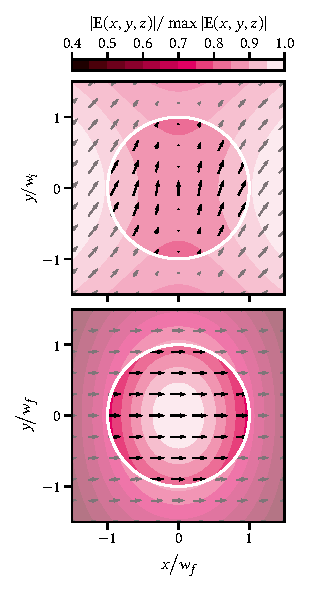
\includegraphics{img/pdf/setup/modes_2d}
    \caption[\imgsource{img/py/setup/extraction.py}]{
        Electric field at the sample surface (top) and the objective lens plane (bottom).
        The white circle indicates the area from which light can be collected, corresponding to the marginal angle $w_i = d\tan\theta_{\mr{m}}$ for the upper and $w_f = \flatfrac{\CA}{2}$ for the lower plot.
        The arrows represent the projection of the vector-valued electric field onto the $xy$-plane.
        At the interface, the polarization is mostly out-of-plane and along $y$, but in the far field, represented by the lens plane, it is almost perfectly polarized along $x$.
        The intensity profile changes from a local minimum at the center to maximal with a roughly circular dependence.
    }
    \label{fig:setup:optics:coupling:modes_2d}
\end{marginfigure}

In order to estimate the fiber coupling efficiency of the light escaping the sample and collected by the objective lens focused by the ocular lens \enquote{D}, we need to consider refraction and transmission of the electric field at the surface, collimation by the objective lens, as well as diffraction at the ocular lens aperture.
A detailed accounting of these effects is beyond the scope of this thesis.
However, let us at least gain an intuition for the degree of these effects.
Since we observe the dipole, oriented in-plane inside the \gls{qw}, from the side, it is useful to rotate the spherical coordinate system so that it is embedded in the coordinate system $(x, y, z)$ as defined in \cref{fig:setup:optics:coupling:emission} with coordinates $(r, \theta, \phi)$.

The magnitude of the electric field vector in the surface plane, which I derive in more detail in \cref{subsec:app:setup:optics:modes}, is shown in the upper panel of \cref{fig:setup:optics:coupling:modes_2d}.
The circle delimits the cone of emission bounded by $\theta_\mr{m}$ (radius $w_i$) while the arrows indicate the projection of the electric field $\bvec{E}(x, y, z)$ onto the interface, indicating that the polarization in the plane points mostly along $y$ at this distance from the source.
Accounting for refraction and modifying the perpendicular and parallel ($s$ and $p$) components of the electric field according to Fresnel's equations~\cite{Hecht2017} results in the electric field in the plane of the objective lens at a distance of $\fob$ shown in the lower panel.
Here, the circle indicates the \gls{ca} of the lens with radius $w_f$.
The picture is quite different from before.
First, the field is almost exclusively polarized along $x$, the dipole axis, as we might have expected.
Moreover, the intensity $\propto\abs{\bvec{E}}^2$ does not depend strongly on the azimuthal angle $\phi$ at this distance, allowing us to approximate the field as rotationally invariant to estimate the coupling efficiency into the \gls{smf}.\sidenote[][*-4]{
    Note that, while a fairly good approximation for the amplitude, this is likely not a good approximation for the phase because $k w_i \sim 1$, meaning that when the light exits the sample the phase is not constant across the surface, and the approximation as a point source just below the surface emitting a spherical wave warrants further investigation, \cf \cref{subsec:app:setup:optics:modes}.
}
As shown in \cref{subsec:app:setup:optics:modes}, the field after collimation is thus to good approximation given by
\begin{equation}\label{eq:setup:optics:coupling:efield:lens}
    \bvec{E}(r, \theta) = \tilde{A}(r)E_x(\theta)
\end{equation}
with
\begin{align}
    \tilde{A}(r) &= \frac{\abs{\bvec{p}}k^2}{4\pi\epsilon}\frac{\exp(\i k z)}{r} \\
    E_x(\theta) &= \frac{2n\pi\cos\theta\left[\cos\theta + n\nu(\theta) + n\nu(\theta)\cos\theta + \nu(\theta)^2\right]}{[n\cos\theta + \nu(\theta)][\cos\theta + n\nu(\theta)]} \label{eq:setup:optics:coupling:efield:lens:x}
\end{align}
and where $\nu(\theta) = \sqrt{1 - n^2\sin^2\theta}$.
For $\tilde{A}(r)$, we assumed a perfect lens that transforms a spherical wave front with constant phase at constant $r$ into a plane wave with constant phase at constant $z$.

\begin{marginfigure}[*-7]
    \centering
    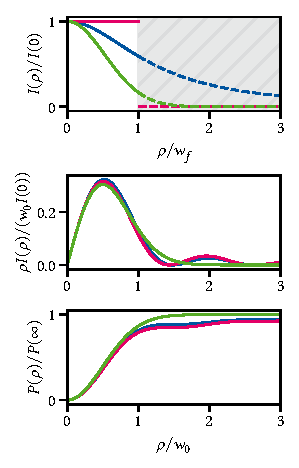
\includegraphics{img/pdf/setup/modes_1d}
    \caption[\imgsource{img/py/setup/extraction.py}]{
        Electric field modes.
        Top: mode intensity of the light collected from the semiconductor at the objective lens plane (blue) in comparison to a flattop (magenta) and Gaussian \TEM{00} mode with theoretical beam diameter after collimating with the ocular lens (green).
        $w_f$ is the lens \gls{ca} radius.
        Middle: diffraction pattern of the collimated beam when focusing onto the \gls{smf} end face with the ocular lens (blue), the flattop approximation (magenta), and the fiber's guiding mode (green).
        The curves are scaled with the radial coordinate $\rho$ to highlight the Airy rings.
        Bottom: power encased by a circle with radius $\rho$, $P(\rho)\propto\int_0^{\rho}\dd{\rho^\prime} \rho^{\prime} I(\rho^{\prime})$.
    }
    \label{fig:setup:optics:coupling:modes_1d}
\end{marginfigure}

The radial intensity profile ($\rho = \fob\tan\theta$ and $r=\sqrt{\rho^2 + \fob^2}$) given by the absolute value square of \cref{eq:setup:optics:coupling:efield:lens} is shown in the upper panel of \cref{fig:setup:optics:coupling:modes_1d} together with a flattop (magenta) and a Gaussian (green) beam profile for comparison.
The intensity drops to about half its maximum at the edge of the lens aperture, $\rho=w$.
We may thus expect the mode matching to be qualitatively different from the flattop behavior discussed previously when coupling this beam into a \gls{smf} with a guiding mode very closely approximating the Gaussian \TEM{00} mode.

The light collected and collimated by the objective lens next passes through the ocular lens in the detection arm which focuses it into the \gls{smf}.
The image of the beam on the fiber end face is given by the Fraunhofer diffraction pattern generated by the wave (\cref{eq:setup:optics:coupling:efield:lens}) incident on the ocular lens aperture, which I give in \cref{subsec:app:setup:optics:diffraction}.
The resulting diffraction pattern, \cref{eq:app:setup:optics:diffraction}, scaled with the radius $\rho$ is plotted in the middle panel of \cref{fig:setup:optics:coupling:modes_1d} together with the corresponding Airy disk result for a flattop beam (\cref{eq:setup:optics:coupling:flattop:diffraction_pattern}) and the \gls{smf}'s guiding Gaussian mode.
The pattern of the flattop and the more accurate mode profile from \cref{eq:setup:optics:coupling:efield:lens} are quite similar, but noticeably differ from the Gaussian mode at higher radii $\rho$.
The lower panel shows the fraction of power included in a circle of radius $\rho$, $P(\rho)\propto \int_0^{\rho}\dd{\rho^{\prime}} \rho^{\prime} I(\rho^{\prime})$, demonstrating that we can expect the mode matching to be fairly good.
Indeed, evaluating \cref{eq:setup:optics:coupling:efficiency:mode_matching} for the light field ($E_{\mr{l}}$, \cref{eq:setup:optics:coupling:efield:lens}) and the fiber's guiding mode ($E_{\mr{g}}$, \cref{eq:setup:optics:coupling:efield:tem00}), results in
\begin{equation}\label{eq:setup:optics:coupling:efficiency:mode_matching:eval}
    \eta_{\mr{m}}(E_{\mr{l}}, E_{\mr{g}})\approx\qty{83}{\percent}
\end{equation}
for our parameters, slightly better than the naive result using the flattop beam.
Together with the collection efficiency (\cref{eq:setup:optics:coupling:efficiency:collection}) and accounting for the transmittance of the \gls{bs}, $\transmittance_{\mr{\acrshort{bs}}}\approx\qty{87}{\percent}$,\sidenote[][*-2]{
    \label{sidenote:setup:optics:bs}
    While the specifications of the beamsplitter are $\transmittance\div\reflectance = \qty{90}{\percent}\div \qty{10}{\percent}$, in reality $\transmittance\div \reflectance\approx\qty{87}{\percent}\div \qty{6}{\percent}$ which also varies slightly with polarization.
}
the \emph{optical efficiency}~\cite{Sze2007} from sample to fiber is thus
\begin{equation}\label{eq:setup:optics:coupling:efficiency:optical}
    \eta_{\mr{o}} = \eta_{\mr{c}}\eta_{\mr{m}} \transmittance_{\mr{\acrshort{bs}}} \approx\qty{1.0}{\percent}.
\end{equation}

\begin{margintable}[*-3]
    \centering
    \footnotesize
    \begin{threeparttable}
        \caption{
            Measured efficiencies of optical elements along the detection path for laser light reflected from the sample.
            All efficiencies are with respect to the previous stage, \ie, the first row is the amount of power measured after \gls{bs}1 divided by the power entering the cryostat
        }
        \label{tab:setup:optics:efficiency:measured}
        \begin{tabularx}{\marginparwidth}{lS}
            \toprule
            \textsc{Opt. element}                   & \multicolumn{1}{c}{\textsc{Efficiency} (\unit{\percent})} \\
            \midrule
            Collection + \acrshort{bs}1\tnote{a}    & 37.8 \\
            Analyzer\tnote{b}                       & 67.6 \\
            Detection fiber\tnote{c}                & 39.1 \\
            Spectrometer\tnote{d}                   & 22.2 \\
            \midrule
            Total                                   & 2.2 \\
            \bottomrule
        \end{tabularx}
        \begin{tablenotes}
            \scriptsize
            \item[a] Reflected and transmitted through windows and \acrshort{bs}1
            \item[b] Transmitted through the analyzer
            \item[c] Emitted from the detection \acrshort{smf}
            \item[d] Emitted from the spectrometer side exit port
        \end{tablenotes}
    \end{threeparttable}
\end{margintable}

Due to the small intensities when dealing with \gls{pl} emitted from a membrane sample, it is difficult to measure this efficiency directly to compare it to the theoretical expectation.
What can be done rather easily is measure the reflected laser power as it is collected by the objective lens.
Together with the reflectance obtained from the calibration measurement in \cref{sec:setup:vibrations:optic}, we can then estimate the various efficiencies.
With the polarizer and analyzer co-polarized for maximum transmission and the laser $s$-polarized \wrt to \gls{bs}1 (\cf \cref{fig:setup:optics:optical_path}), I measured the efficiencies listed in \cref{tab:setup:optics:efficiency:measured}.
The \enquote{Collection + \gls{bs}1} efficiency corresponds to $\transmittance_{\mr{\acrshort{bs}}}\reflectance_{\mr{S}}$ with $\reflectance_{\mr{S}}$ the reflectance of the sample and matches reasonably well the expected value of $\reflectance_{\mr{S}}=\abs{(n-1)/(n+1)}^2\approx\qty{32}{\percent}$ for \ch{GaAs}.
In \cref{sec:exp:tmm}, I analyze the reflectance of membrane samples in more detail using \gls{tmm} simulations and find thin-film interference effects should should actually decrease the bare sample reflectance around \qty{20}{\percent}.
The transmittance of the analyzer (a nanoparticle linear film polarizer~\cite{ThorlabsLPVIS050-MP2}) is lower than expected from the datasheet, which quotes around \qty{80}{\percent} at \qty{800}{\nano\meter}.
Coupling into the \gls{smf} (\enquote{Detection fiber}) is significantly worse than expected from the considerations in \cref{subsec:setup:optics:coupling:lenses} for a Gaussian beam.
Since the beam used to measure the efficiencies is launched from and collimated by the same fiber type and lens as used to collect the light, the coupling efficiency should theoretically be as large as unity.
However, due to the small \gls{mfd}, alignment is tricky and vibrations may be expected to significantly reduce the coupling efficiency (\cf \cref{ch:setup:vibrations}).
It is moreover unclear how well the beam retains its Gaussian \TEM{00} mode profile after traversing the entire optical path (\cf \cref{fig:setup:optics:optical_path}).
Lastly, the throughput efficiency of the spectrometer is also lower than expected by a factor of order two, albeit still an improvement over the \qty{12}{\percent} reported in \citer{Descamps2021}.
The gratings have efficiencies on the order of \qty{50}{\percent}, and since the measurement was conducted with monochromatic light, there should be no other significant loss channels, indicating the spectrometer might not be perfectly well aligned.\sidenote{
    Note that the spectrometer has an adjustable input slit that can be used to limit the spot size and thereby improve the resolution at the cost of reducing overall intensity.
    However, I have found this not to have a significant impact because the \gls{smf} already has a very small \gls{mfd} and there is little to no improvement from further decreasing it.
}
To fully account for all losses, the \gls{pde} (also called \gls{qe}) of the \gls{ccd} (\theccd, $\eta_{\QE}\sim\qty{85}{\percent}$) or the \glspl{spcm} (\thespcm, $\eta_{\QE}\sim\qty{65}{\percent}$) needs to be taken into account.
In summary, while certainly allowing room for improvement, the total optical efficiency of $\eta_{\mr{o,tot}} = \qty{2.2}{\percent}$ given by the power arriving at the plane of measurement -- either the \gls{ccd} or the \glspl{spcm} -- as fraction of the power incident on the cryostat is at an acceptable level.

\subsection{Imaging the laser spot}\label{subsec:setup:optics:coupling:imaging}
As the confocal microscope is free space, we are in a position to image the sample using a white light source.
We can also, though, use the imaging capabilities to inspect the laser spot focused onto the sample and compare it to the behavior expected from \cref{subsec:setup:optics:coupling:lenses}.
To this end, I coupled the laser into both excitation and detection arm of the microscope and aligned their spots on top of each other on a gold gate fabricated using optical lithography -- ensuring close to perfect reflectivity -- by monitoring their image on the \cmoscam (\cf \cref{fig:setup:optics:optical_path}).
A feature of known size, for example the width of the gate, can be used to calculate the magnification of the lens system defined by O and C (\cf \cref{sec:setup:vibrations:optic}).\sidenote{
    Note that this varies slightly depending on the focal distance of sample and camera from their respective lenses.
    Theoretically, we expect the magnification to be given by the ratio of their focal lengths, $M=\foc/\fob\approx\num{32}$.
}
Once aligned and blocking the beam from each arm in turn, I recorded a picture of the spots.

\begin{figure}
    \centering
    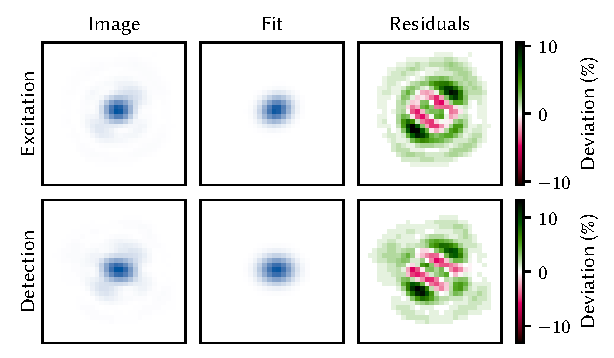
\includegraphics{img/pdf/setup/spots}
    \caption[\imgsource{img/py/setup/imaging.py}]{
        Imaging of the laser spots using the free-space imaging capabilities of the confocal microscope.
        Left column shows cropped images of the spot on an optical gate taken with the \gls{cmos} camera, while the middle column shows the fit to \cref{eq:setup:optics:coupling:intensity:tem00} rotated by a variable amount.
        Right column shows the residuals of the fit, highlighting non-Gaussian components in the beam.
        Top row is the excitation, bottom the detection path.
    }
    \label{fig:setup:optics:coupling:imaging}
\end{figure}

From \cref{eq:setup:optics:coupling:efield:tem00}, we can deduce that a perfect, aberration-free spot would have the two-dimensional intensity distribution
\begin{equation}\label{eq:setup:optics:coupling:intensity:tem00}
    I(x, y) = I(0, 0) \exp\left\lbrace -\frac{2 x^2}{w_{0,x}^2} -\frac{2 y^2}{w_{0,y}^2} \right\rbrace,
\end{equation}
where $w_{0,x(y)}$ are the beam waist radii in $x$ and $y$-direction, respectively, which are equal in the perfect case and introduce ellipticity else.
Allowing for ellipticity as well as a rotation of the coordinate system with respect to the axes of the \gls{cmos} camera, we can fit \cref{eq:setup:optics:coupling:intensity:tem00} to the pictures obtained previously.
The result is shown in \cref{fig:setup:optics:coupling:imaging} for the excitation path in the upper and the detection path in the lower row.
The first column shows a cropped section of the recorded images, showing good alignment (large overlap) between both spots but also some sidelobes along perpendicular axes rotated by around \qty{45}{\degree} to the camera axes.
This is also reflected in the relative residuals of the fitted spot that clearly shows that the spot is not described only by a Gaussian \TEM{00} mode.
However, extracting the beam waist radii from the fits and scaling with the magnification factors, which display a slight asymmetry between the two axes, \num{30} to \num{27.4}, we obtain reasonable results between \num{1.4} and \num{2} times larger than the diffraction limit given by the lens geometries, \cf \cref{subsec:setup:optics:coupling:lenses}, as shown in \cref{tab:setup:optics:coupling:imaging}.
For a more faithful measurement of the spot size one typically performs a knife-edge measurement.
This has the advantage that it does not depend on additional components of the optical path such as the beam splitter \acrshort{bs}2 and focusing lens.
In \cref{sec:setup:vibrations:optic} I perform such a measurement in the context of vibration spectroscopy.

\begin{margintable}
    \centering
    \footnotesize
    \caption{
        Beam waist radii extracted from the fits of \cref{eq:setup:optics:coupling:intensity:tem00} to the images recorded using the imaging path of the confocal microscope.
    }
    \label{tab:setup:optics:coupling:imaging}
    \begin{tabular}{lSS}
        \toprule
        \textsc{Beam waist} (\unit{\micro\meter})    & $w_{0, x}$ & $w_{0, y}$ \\
        \midrule
        Detection path                               & 0.58       & 0.75 \\
        Excitation path                              & 0.60       & 0.84 \\
        Diffraction limit                            & 0.42       & 0.42 \\
        \bottomrule
    \end{tabular}
\end{margintable}

From experience, the sidelobes present in \cref{fig:setup:optics:coupling:imaging} can be suppressed with better alignment and are most likely due to an imperfect focal distance of the fiber collimating lenses D and E resulting in a secondary (back) focal plane before the objective lens.
The asymmetry resulting in elliptical spot cross sections, on the other hand, might be due to several factors including a tilt of the sample or alignment of the imaging arm of the microscope.\sidenote{
    Notice that the asymmetry is due solely to the magnification factor rather than the image on the camera,
}
Finally, note that the excitation spot typically looks worse than the detection spot, likely because of the additional optical elements introducing beam distortions.

\subsection{Cross-polarization extinction}\label{subsec:setup:optics:coupling:rejection}
An essential part of the confocal microscope's design is the ability to reject the excitation laser from coupling into the detection fiber.
In a conventional microscope, this issue is avoided because one can arrange the illumination and detection lenses such that their optical axes are orthogonal and the light used for excitation of the sample does not scatter into the objective lens.
In a confocal geometry, though, the same lens is used for excitation and detection, and unwanted excitation light dominates the response unless filtered out by means of, \eg, a notch filter.
This limits the optical bandwidth of the microscope and hence other techniques are desirable.
Here, excitation rejection is achieved by cross-polarization of the polarizer (P, \polarizer) setting the polarization axis of the beam launched from the excitation \gls{smf} and the analyzer (A, \polarizer) just before coupling the light into the detection \gls{smf}.
As demonstrated by \citet{Benelajla2021}, this technique enables extinction ratios\sidenote{
    Defined as incident power over transmitted power.
}
up to \num{1e10} in a confocal geometry, far beyond the bare polarizer extinction ratio of up to $\sim\num{1e8}$~\cite{ThorlabsLPVIS050-MP2}.
In our case, vibrations and rough sample surfaces off which the light is reflected limit the extinction ratio to $\sim\num{1e6}$.

As the laser beam launched from the excitation fiber is already polarized, rather than rotate the polarizer, the plane of polarization is rotated using a \halfwave plate.
To compensate for ellipticities introduced by the \gls{bs}, windows, and sample reflection, a \quarterwave plate is inserted after the \halfwave plate~\cite{Kuhlmann2013}.
The waveplates are mounted on piezoelectric rotation stages (\rotator with \rotatorcontroller controller), allowing for computer-controlled adjustment of the angles.
Previously, a third rotation stage was used to rotate the analyzer, but I found this to deteriorate the fiber coupling, most likely due to an angle-dependent beam deflection of the analyzer.\sidenote{
    This effect was less pronounced with the unmounted version of the same polarizer, \polarizerunmounted.
    That though introduced significant etaloning with a free spectral range of $\Delta\lambda\approx\lambda^2/2 n l\approx\qty{100}{\pico\meter}$ matching the substrate thickness of $l = \qty{2}{\milli\meter}$~\cite{Ismail2016}.
}
Furthermore, the optics behind the analyzer such as the diffraction grating have polarization-dependent properties so that it is in any case a good idea to fix the plane of polarization of the detection path after the analyzer.
I therefore used only the waveplates on the excitation arm to fine-tune the excitation rejection, which is not ideal since the same argument as before naturally also applies to the optics behind these, such as the beam splitter whose ratio is polarization dependent.
It is hence advisable to insert another \halfwave plate on a rotation stage before the analyzer and use it together with the \quarterwave plate for rejection control as indicated in \cref{fig:setup:optics:optical_path}.

To analyze the properties of the excitation rejection, I measured the \gls{od} as a function of the relative waveplate angles $\Delta\phi_{\halfwave(\quarterwave)}$.
The \gls{od} is defined as
\begin{equation}\label{eq:setup:optics:od}
    \OD = \log_{10}\left(\frac{P_{\mr{i}}}{P_{\mr{t}}}\right) = \log_{10}\left(\frac{1}{\transmittance}\right),
\end{equation}
where $P_{\mr{t}}$ is the transmitted power after, $P_{\mr{i}}$ the incident power before the analyzer, and \transmittance the transmittance of the analyzer.
To evaluate this expression, I measured the photon flux $\dot{\Phi}_{\mr{t}}$ after the spectrometer using the \glspl{spcm} when irradiating a sample with the laser and compared it to the power $P$ measured at the optical head.
Together with the optical efficiency $\eta_{\mr{o,tot}}$ measured in \cref{subsec:setup:optics:coupling:efficiency}, the \gls{spcm}'s \gls{pde} $\eta_{\QE}$, and the beam splitter ratio $\transmittance\div\reflectance$ (\cf \cref{sidenote:setup:optics:bs}), \cref{eq:setup:optics:od} then becomes
\begin{equation}\label{eq:setup:optics:od:eval}
    \OD = \log_{10}\left(\frac{P\times\flatfrac{\reflectance}{\transmittance}}{\flatfrac{hc}{\lambda}\times\dot{\Phi}_{\mr{t}}/\eta_{\mr{o,tot}}\eta_{\QE}}\right).
\end{equation}

\begin{figure}
    \centering
    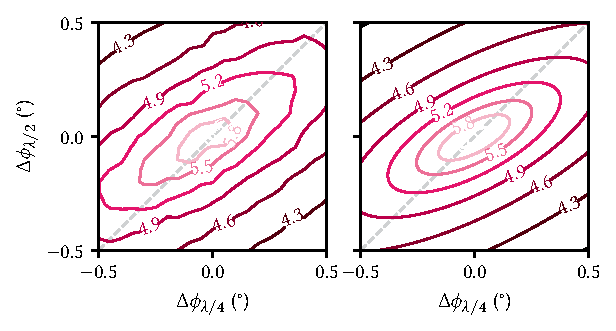
\includegraphics{img/pdf/setup/rejection}
    \caption[\imgsource{img/py/setup/excitation_rejection.py}]{
        \Gls{od} measured (left) and fitted (right) as function of relative \quarterwave and \halfwave angles.
        The dashed gray line indicates the axis along which there should be no dispersion if all optics between polarizer and analyzer were polarization-independent.
    }
    \label{fig:setup:optics:rejection}
\end{figure}

\Cref{fig:setup:optics:rejection} shows a measurement for which the laser was focused on an exciton trap (\cf \cref{part:exp}) in the left panel.
The dashed gray line indicates the axis along which the \gls{od} should theoretically be constant (rotating the \halfwave plate changes the plane of polarization, so the \quarterwave plate should need to be rotated by the same amount to retain a constant angle between plane of polarization and fast axis of the waveplate).
The \gls{od} reaches maximum values around \num{6.4} -- corresponding to an extinction ratio of \num{2.5e6} -- but quickly falls off by more than an order of magnitude even for small angular displacements.\sidenote{
    The maximum achievable \gls{od} depends strongly on the sample surface off which the laser is reflected, see also \citer{Kumar2016}.
}
Qualitatively, one finds that close to the extinction maximum (maximal \gls{od}), the count rate $\dot{\Phi}_{\mr{t}}$ is a rotated paraboloid of the form
\begin{equation}
    \dot{\Phi}_{\mr{t}} = \bvec{a}\transpose\bvec{\Delta\tilde{\phi}}^2 + \dot{\Phi}_0
\end{equation}
with $\bvec{\Delta\tilde{\phi}} = R(\pi/4+\theta)\bvec{\Delta\phi}$, $\bvec{\Delta\phi} = (\Delta\phi_{\quarterwave},\Delta\phi_{\halfwave})\transpose$ and $R(\theta)$ a rotation matrix.
Inserting into \cref{eq:setup:optics:od:eval} yields
\begin{equation}\label{eq:setup:optics:od:fit}
    \OD = \log_{10}\left(\frac{P \reflectance\lambda\eta_{\mr{o,tot}}\eta_{\QE}}{h c}\right) - \log_{10}(\bvec{a}\transpose\bvec{\Delta\tilde{\phi}}^2 + \dot{\Phi}_0),
\end{equation}
a fit to which is shown in the right panel of \cref{fig:setup:optics:rejection}, displaying good agreement with the data.
From the fit, we extract $\theta=\qty{-17}{\degree}$, indicating a non-negligible polarization dependence, as well as quadratic dispersion coefficients $\partial^2\OD/\bvec{\Delta\tilde{\phi}}^2=\qty[per-mode=symbol]{-0.16}{\per\milli\txtdegree\squared}$ and \qty[per-mode=symbol]{-0.02}{\per\milli\txtdegree\squared} perpendicular (parallel) to the axis along $\flatfrac{\pi}{4}+\theta$, respectively.

The optics between polarizer and analyzer furthermore display chromatic dispersion.
When changing the excitation wavelength, the angles of \halfwave and \quarterwave plate therefore need to be re-optimized.
I describe the automatic calibration procedure implemented in the measurement framework to this end in \cref{subsec:sec:exp:mjolnir:calibration:rejection}.

\section{Exemplary measurement of non-classical light}\label{sec:setup:optics:g2}
As a demonstration of the optical capabilities of the setup, I performed second-order coherence measurements of an \ch{InAs} \gls{saqd} in \ch{GaAs}.
\Glspl{saqd} are \glspl{oaqd} that form at random locations during epitaxial growth.
They have demonstrated excellent optical properties and show potential for technological applications such as quantum repeaters~\cite{Petroff2001,Warburton2013,Lodahl2015,Zajac2025}.
In particular, \glspl{saqd} can be operated as single-photon sources.
Because they locally deform the band structure, they can capture and confine excitons.
Owing to their small spatial extents, strong Coulomb interaction shifts the energy of excitonic complexes other than the neutral exciton $X^{0}$, implying that light emitted at $h\nu = E_{X^{0}}$ upon recombination is certain to contain a single photon within a time window on the scale of the exciton lifetime.
This so-called photon \emph{anti-bunching} behavior\sidenote{
    Also known as sub-Poissonian statistics.
}
can be measured with a \gls{hbt} interferometer and serves as a fingerprint of single-photon source behavior.

The \gls{hbt} interferometer consists of a symmetric ($\transmittance :\reflectance=\num{50}:\num{50}$) \acrlong{bs} with \glspl{spcm} on each exit port.
Photons incident on the \gls{bs} will be transmitted and reflected with equal probability, and either the detectors at each output will register the photons (a \enquote{click}).
If the distribution of arrival times of the incident photons is Poissonian, the times at which the two detectors will click will be uncorrelated, and hence the distribution of time differences between clicks on either detector will be uncorrelated as well.
This is the classical case.
In the case of sub- or super-Poissonian photon statistics, the click rate will be reduced or enhanced for a time difference at zero, implying that two photons are less or more likely to arrive at the same time, respectively.
The latter case corresponds to thermal light and \emph{photon bunching}.
Here, two photons are more likely to arrive in pairs at exactly the same time.
The former case is that of a single-photon source; once it has emitted a photon, a finite amount of time will pass before it can emit another, and hence the two detectors can never register a click at the same time.

\begin{marginfigure}
    \centering
    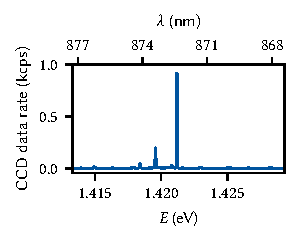
\includegraphics{img/pdf/setup/ingaas_pl}
    \caption[\imgsource{img/py/setup/g2.py}]{
        \Gls{pl} spectrum of a \gls{saqd} under \gls{cw} excitation at \qty{793}{\nano\meter}.
    }
    \label{fig:setup:optics:ingaas:pl}
\end{marginfigure}

I loaded and cooled down an \ch{InAs/GaAs} chip with \glspl{saqd} and selected a bright and isolated emission line.
A typical \gls{pl} spectrum under \gls{cw} above-gap excitation is shown in \cref{fig:setup:optics:ingaas:pl}.
The brightest line at $\qty{1.4212}{\eV} = \qty{872.39}{\nano\meter}$ has a width of around $\qty{15}{\micro\eV} = \qty{12}{\pico\meter}$, close to the grating\sidenote{
    \qty{1800}{gr\per\milli\meter}, resulting in a spectral dispersion of $\dv*{\lambda}{x} = \qty{325}{\pico\meter\per\milli\meter}$ in the focal plane.
}
resolution limit of around \qty{5}{pm}.
To perform a \g2 experiment, light emitted by the source is spectrally filtered using the \thespectrometer diffraction grating spectrometer and sent through a 50:50 \gls{bs} with an \thespcm \gls{spcm} on each exit port.
The clicks from the detectors are time-correlated using a counting card (\tagger), computing the second-order correlation function~\cite{Kimble1976,Walls1979,Cohen-Tannoudji1998}
\begin{equation}
    \g{2}(\tau) = \frac{\expval{\hat{n}_1(t)\hat{n}_2(t + \tau)}}{\expval{\hat{n}_1(t)}\expval{\hat{n}_2(t)}},
\end{equation}
where $\hat{n}_i(t) = \hat{b}^\dagger_i(t) \hat{b}_i(t), i\in\lbrace 1,2\rbrace$ is the photon-number operator for a single mode at detector $i$ and averaging takes place over time.
For a weakly excited artificial atom and in the absence of dephasing, one expects this function to take on the form~\cite{Walls1979,Loudon2000,Grandi2016}
\begin{equation}\label{eq:setup:optics:g2:explicit}
    \g{2}(\tau) = \left[1 - \exp(-\flatfrac{\tau\gamma}{2})\right]^2,
\end{equation}
where $\gamma$ is the Einstein $A$ coefficient, \ie, the spontaneous emission rate or inverse lifetime $T_1\inverse$ of the excited state.
Because $T_1$ is on the order of \qty{1}{\nano\second} for these dots, the detector response time (dominated by the timing resolution of the \gls{spcm}, $\sigma_{\mr{SPCM}} = \qty{350}{\pico\second}$) plays a significant role in the measurement, and one typically fits a convolution of \cref{eq:setup:optics:g2:explicit} with the \gls{irf} of the optical setup to the data instead.
Ideally, the \gls{irf} would be measured using a pulsed laser source.
In the absence of this data, we instead make due with the assumption that the \gls{irf} is dominated by Gaussian timing jitter with $\sigma = \sqrt{2}\sigma_{\mr{SPCM}} \approx \qty{500}{\pico\second}$, where $\sigma_{\mr{SPCM}}$ is the timing resolution quoted in the \gls{spcm} data sheet and the factor of $\sqrt{2}$ is due to the fact that the variance from both \glspl{spcm} adds quadratically.\sidenote[][*-7]{
    Realistically, the true \gls{irf} of the \glspl{spcm} will be some asymmetric rather than a symmetric normal distribution.
    This was also observed in the pulsed Stark-shift experiment in \citer{Descamps2023}.
}
The convolution then becomes
\begin{align}
    \tilde{g}\gth{2}(\tau) &= \frac{1}{\sigma\sqrt{2\pi}}\int\dd{\tau^\prime} g\gth{2}(\tau^\prime)\e^{-\left(\tau - \tau^\prime\right)^2/2\sigma^2} \notag \\
                           &= 1 - 2 K_{\flatfrac{\gamma}{2}}(\tau) + K_{\gamma}(\tau) \label{eq:setup:optics:g2:fit}
\end{align}
with
\begin{align}
    K_\alpha(\tau) &= \e^{\frac{\alpha^2\sigma^2}{2}}\left\lbrace
        \e^{-\alpha\tau}\Phi\left(\frac{\tau - \alpha\sigma^2}{\sigma}\right)
        + \e^{\alpha\tau}\left[1 - \Phi\left(\frac{\tau + \alpha\sigma^2}{\sigma}\right)\right]
    \right\rbrace
\end{align}
where $\Phi(z) = (\flatfrac{1}{2})\left[1 + \erf\left(z/\sqrt{2}\right)\right]$ is the the Gaussian cumulative distribution function.

\begin{marginfigure}[*-15]
    \centering
    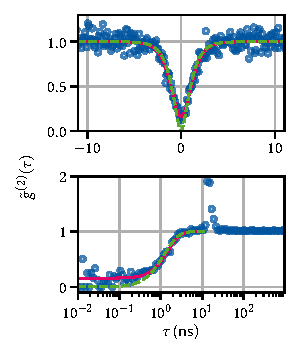
\includegraphics{img/pdf/setup/ingaas_g2}
    \caption[\imgsource{img/py/setup/g2.py}]{
        \g{2} measurement of the emission line at \qty{872.267}{\nano\meter} under \gls{cw} excitation with \qty{1}{\micro\watt} at \qty{793}{\nano\meter}.
        The monochromator bandwidth was $\Delta\lambda = \qty{200}{\pico\meter} = \qty{325}{\micro\eV}$.
    }
    \label{fig:setup:optics:ingaas:g2}
\end{marginfigure}

The upper panel of \cref{fig:setup:optics:ingaas:g2} shows the measurement after a total run time of around \qty{17}{\hour} together with a fit to \cref{eq:setup:optics:g2:fit} (magenta line) from which we extract a lifetime of $\gamma\inverse = \qty{430+-11}{\pico\second}$.
The dashed orange line is the deconvoluted function (\cref{eq:setup:optics:g2:explicit}).
The lower panel shows the same measurement for logarithmically spaced time lags $\tau$ covering a wider range.
A peculiar feature shows at $\tau = \qty{13.4}{\nano\second}$, where the measurement suggests a bunching of photons with $\g2(\tau) \approx 2$.
The origin of this bump is not understood.
One possible cause might be multiple reflections in the setup.
However, in free space the delay corresponds to a time-of-flight distance of \qty{4}{\meter}, far larger than any distances in the setup besides the path between objective and ocular lens at $\sim\qty{1.5}{\meter}$.
Assuming a refractive index of $n=\num{1.4}$ for a typical \gls{smf} results in a characteristic distance of \qty{2.8}{\meter} which also does not match any components in the setup.\sidenote{
    The closest match is the \qty{10}{\meter} fiber from the optical head to the optical table.
}
What can be said is that it is related to the setup rather than a physical process in the sample since the feature also appeared in \g2 measurements on different samples.
For measurements such as the one performed here, though, this effect may safely be treated as a measurement artefact and ignored.
Only in case the characteristic decay time $\gamma\inverse$ approached \qty{10}{\nano\second} this would need to be investigated more carefully.
Finally, I note that the dependence of the integrated peak power on excitation power for this line was superlinear, suggesting an excitonic complex rather than the neutral exciton as the source of emission.
The line at \qty{1.4196}{\eV} did show a linear relationship and produced qualitatively the same \g2 results.
